\textcolor{black}{\section{Resultados y Análisis}}

{\subsection{Dy$^{3+}$ en un ambiente de fosfato de magnesio}
\noindent Se muestra a continuación el espectro de emisión del ion de disprosio en una matriz vítrea de fosfato de magnesio: 
\begin{figure}[H]
    \centering
    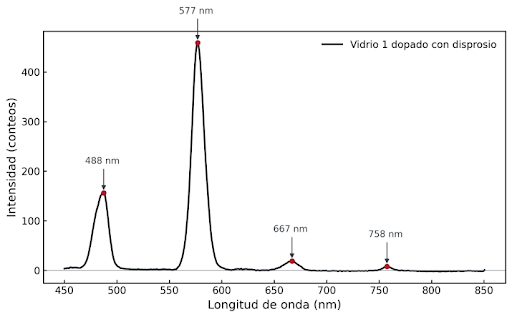
\includegraphics[scale=0.42]{disprosio_fosfato.png}
    \caption{Espectro de emisión del fosfato de magnesio dopado con un ion trivalente de disprosio}
    \label{fig:placeholder}
\end{figure}
Observamos que prresenta 4 máximos de intensidad localizados alrededor de $487.5\pm 16$ nm, $577\pm 14$ nm, $667 \pm 16$ nm, $758 \pm 9$ nm. Las bandas de mayor intensidad se presentan en $488 \pm 8$ nm que corresponde al color azul y $577\pm 14$ nm que corresponde al color amarillo. Mientras que las bandas de menor intensidad se observan en $667 \pm 16$ nm y $758 \pm 9$ nm. A partir de estas longitudes de onda, se calcularon los números de onda correspondientes mediante

\begin{equation}
    \tilde{\nu} = \frac{10^{7}}{\lambda}
\label{eq:numero_onda}
\end{equation}

obteniéndose $(20513 \pm 1348)\,\text{cm}^{-1}$, $(17331 \pm 841)\,\text{cm}^{-1}$, $(14993 \pm 742)\,\text{cm}^{-1}$, $(13201 \pm 314)\,\text{cm}^{-1}$. Estos valores están asociados a las diferencia de energía observadas. A continuación, se muestra un gráfico de la energía asociada a cada longitud de onda: 
\begin{figure}[H]
    \centering
    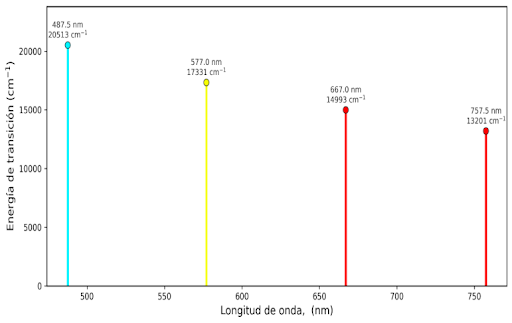
\includegraphics[scale=0.45]{figs/niv_energia_fosfato_magnesio.png}
    \caption{Energías asociadas a las diferencias de energía entre niveles. Se observa la energía correspondiente a cada longitud de onda}
    \label{fig:placeholder}
\end{figure}
El máximo de menor longitud de onda observado en el espectro de emisión está asociado a una mayor energía, mientras que el máximo de mayor longitud de onda corresponde a una menor energía de transición entre niveles. El diagrama de niveles para el ion de disprosio en fosfato de magnesio muestra transiciones radiativas desde el nivek $^4F_{9/2}$ del ion Dy$^{3+}$ hacia niveles de menor energía. La transición de menor longitud de onda, $(488 \pm 8)\,\text{nm}$ , termina en el estado fundamental  $^6H_{15/2}$ y corresponde a la mayor energía de emisión  $(20513 \pm 1347)\,\text{cm}^{-1}$. Las transiciones de asociadas a luz registrada para las longitudes de onda restantes terminan en niveles más altos t energías menores. Esto corresponde a la relación inversa entre la longitud de onda de la radiación y su energía.
\begin{figure}[H]
    \centering
    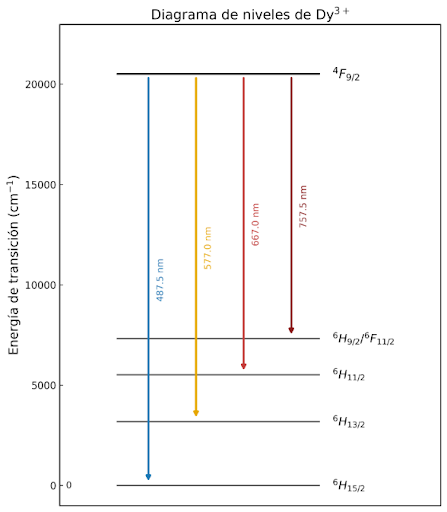
\includegraphics[scale=0.45]{figs/diagrama de niveles.png}
    \caption{Niveles de transición del Dy$^{3+}$}
    \label{fig:placeholder}
\end{figure}
{\subsection{Disprosio en un cristal de metafosfato de magnesio}
\begin{figure}[ht]
  \centering
  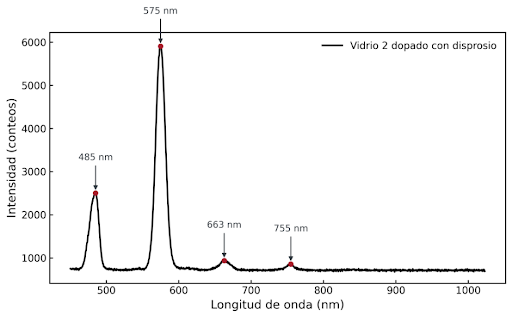
\includegraphics[scale=0.45]{disprosio_metafosfato.png}

  \medskip

  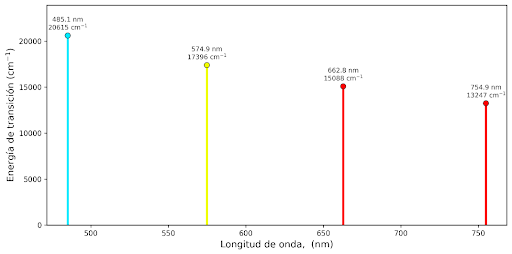
\includegraphics[scale=0.45]{energias_metafosfatos_2.png}
  \caption{Espectro de emisión del disprosio incorporado en metafosfato (Vidrio de metafosfato de zinc, Zn(PO$_3$)$_2$, dopado con óxido de disprosio (Dy$_2$O$_3$) al 1\%.) de magnesio y energía asociadas a cada longitud de onda detectada}
\end{figure}
El espectro de emisión presenta 4 bandas procipales, con máximos en $485. 1\pm 9.2\,\text{nm}$, $574.9\pm 10\,\text{nm}$, $662.8\pm 10\,\text{nm}$, $754.9\pm 9\,\text{nm}$. La banda centrada en $574.9\pm 10\,\text{nm}$ presenta la mayor intensidad, alrededor de 5900 cuentas. Se puede observar que la  emisión más intensa está localizada en la región del amarillo y se asocia a la transición de $^4F_{9/2}\rightarrow{}^6H_{13/2}$ del ion $Dy^{3+}$. Las demás bandas se deben a transiciones del nivel $^4F_{9/2}$ a niveles de menor energía. A continuación se muestra el diagrama de niveles de energía: 
\begin{figure}[H]
    \centering
    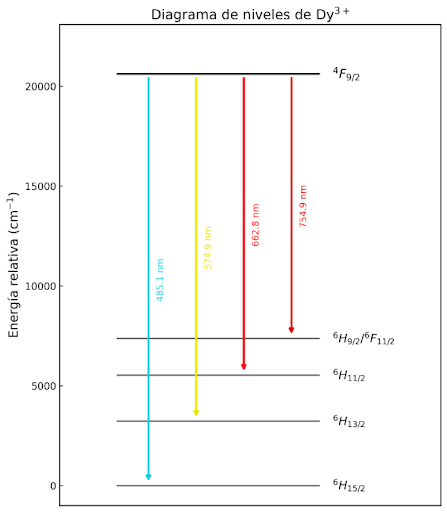
\includegraphics[scale=0.45]{figs/disgramas_metafosfato.png}
    \caption{Diagrama de niveles de Dy$_2$O$_3$) al 1\% en un vidrio de metafosfato de zinc, Zn(PO$_3$)$_2$}
    \label{fig:placeholder}
\end{figure}
 
Al comparar los espectros de emisión del ion de disprosio en los distintos ambientes, tenemos lo siguiente: 
\begin{figure}[H]
    \centering
    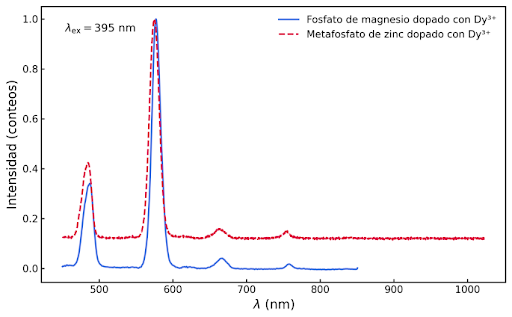
\includegraphics[scale=0.45]{figs/dos_espectros.png}
    \caption{Comparación de los dos espectros de emisión obtenidos a partir del ion de disprosio en distintos ambientes}
    \label{fig:placeholder}
\end{figure}

Las diferencias observadas pueden relacionarse con el ambiente químico que proporciona cada matriz al ion Dy$^{3+}$.

{\subsection{Samario en un ambiente de fosfato de zinc}
\noindent 
El espectro de emisión del vidrio de fosfato de zinc dopado con Sm$_2$O$_3$
presenta cuatro bandas principales, con máximos aproximados en $566.0 \pm 13.5$, $602.5 \pm 14$,
$648 \pm 14$ y $708\pm 20\,\text{nm}$. La banda de 602\,\text{nm} es la más intensa,
con un máximo cercano a 185 cuentas. Las bandas de $648 \pm 14$ y  $566.0 \pm 13.5 $\,\text{nm}
alcanzan intensidades aproximadas de 110 y 70 cuentas, respectivamente,
mientras que la banda de $708.5\pm 20.5$\,\text{nm} es débil, con una intensidad
cercana a 7 cuentas.

\begin{figure}[ht]
  \centering
  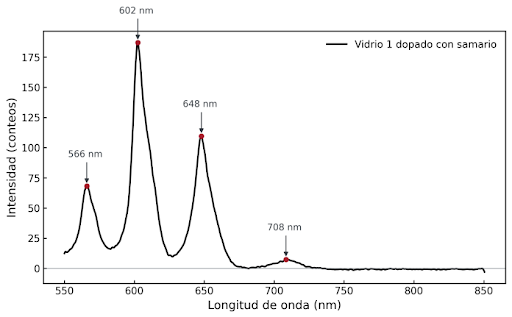
\includegraphics[scale=0.45]{figs/samario_espectro.png}

  \medskip

  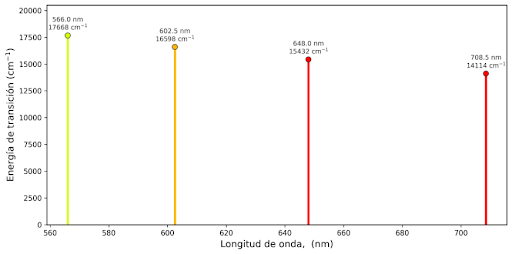
\includegraphics[scale=0.45]{figs/energia_samario_1.png}
  \caption{Espectro de emisión del vidrio de fosfato de zinc,
Zn(PO$_3$)$_2$:Zn$_3$(PO$_4$)$_2$, dopado con óxido de samario
(Sm$_2$O$_3$), y energías asociadas a las longitudes de onda detectadas.}
\end{figure}
El espectro de emisión del vidrio de fosfato de zinc dopado con Sm$_2$O$_3$
presenta bandas en $566.0 \pm 13$ , $602.5 \pm 14$, $648.0 \pm 14 $ y $708.5 \pm 20.5\,\text{nm}$. La banda de
$602.5\,\text{nm}$ es la más intensa y la de $708.5\,\text{nm}$, la menos
intensa. Los números de onda correspondientes son $17668\pm 843.3 $, $16598\pm 771.7$, $15432\pm 667$ y $14114\pm  817\,\text{cm}^{-1}$, respectivamente. Las emisiones se asignan a transiciones desde $^4G_{5/2}$ hacia los niveles $^6H_{5/2}$, $^6H_{7/2}$, $^6H_{9/2}$ y $^6H_{11/2}$ del Sm$^{3+}$.
\begin{figure}[H]
    \centering
    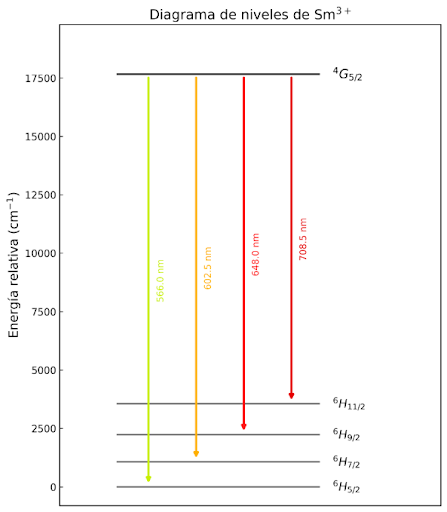
\includegraphics[scale=0.45]{figs/diagrama de niveles_samario.png}
    \caption{Diagrama de niveles para Sm$_2$O$_3$ en un ambiente de vidrio de fosfato de zinc (Zn(PO$_3$)$_2$:Zn$_3$(PO$_4$)$_2$) }
    \label{fig:placeholder}
\end{figure}
{\subsection{Samario en un ambiente de fosfato de zinc - medidas con un segundo aparato de medición}
\begin{figure}[ht]
  \centering
  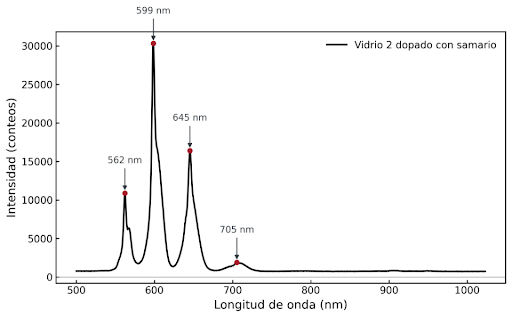
\includegraphics[scale=0.45]{figs/espectro_samario_2.png}

  \medskip

  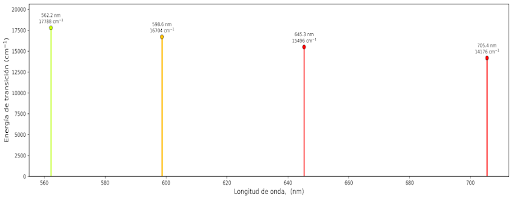
\includegraphics[scale=0.45]{figs/samario_energias_aparato_2.png}
  \caption{Espectro de emisión del vidrio de fosfato de zinc,
Zn(PO$_3$)$_2$:Zn$_3$(PO$_4$)$_2$, dopado con óxido de samario
(Sm$_2$O$_3$), y energías asociadas a las longitudes de onda detectadas (con un segundo aparato de medición).}
\end{figure}
El espectro obtenido con el espectrómetro \textit{Ocean Optics}  presenta bandas alrededor
de $562.2\pm 9.5$, $598.6\pm 0.3$, $645\pm 0.3$ y $705.4\pm 41.2\ ,\text{nm}$, asignadas a transiciones del Sm$^{3+}$
desde $^4G_{5/2}$ hacia $^6H_{5/2}$, $^6H_{7/2}$, $^6H_{9/2}$ y
$^6H_{11/2}$, respectivamente. Estas posiciones son cercanas a las del
primer aparato, en concordancia con la
medición del mismo material. Las pequeñas diferencias pueden relacionarse
con la resolución o calibración de los equipos. La banda cercana a
$598.6\pm 0.3 \,\text{nm}$ es la más intensa en esta medición; las intensidades
absolutas no se comparan directamente entre aparatos porque pueden
depender de sus condiciones de detección. Los números de onda calculados
son aproximadamente $17788\pm 602$, $16704\pm 19.6 $, $15496\pm 16.3 $ y $14176\pm 1664 \,\text{cm}^{-1}$.
%%%%% TERBIO %%%%%%%%%%%%%%%%%%%%%%%%%%%%%%%%%%%%%%%%%%%%%%

{\subsection{Terbio en un cristal de tetraborato de litio}
\noindent En la Figura \ref{fig:Tb_espectro} se muestra su espectro de emisión. Se consideraron como bandas de mayor intensidad a las intensidades máximas de la gráfica más una incertidumbre, calculada como el ancho de la mitad de la intensidad máxima correspondiente. Por tanto, se obtuvieron los siguientes valores: $\lambda_{Tb_1} = 492.0 \pm 18.00$ nm, $\lambda_{Tb_2} = 547.5 \pm 11.50$ nm, $\lambda_{Tb_3} = 590.0 \pm 16.50$ nm y $\lambda_{Tb_4} = 625.5 \pm 12.50$ nm.

\begin{figure}%[H]
    \centering
    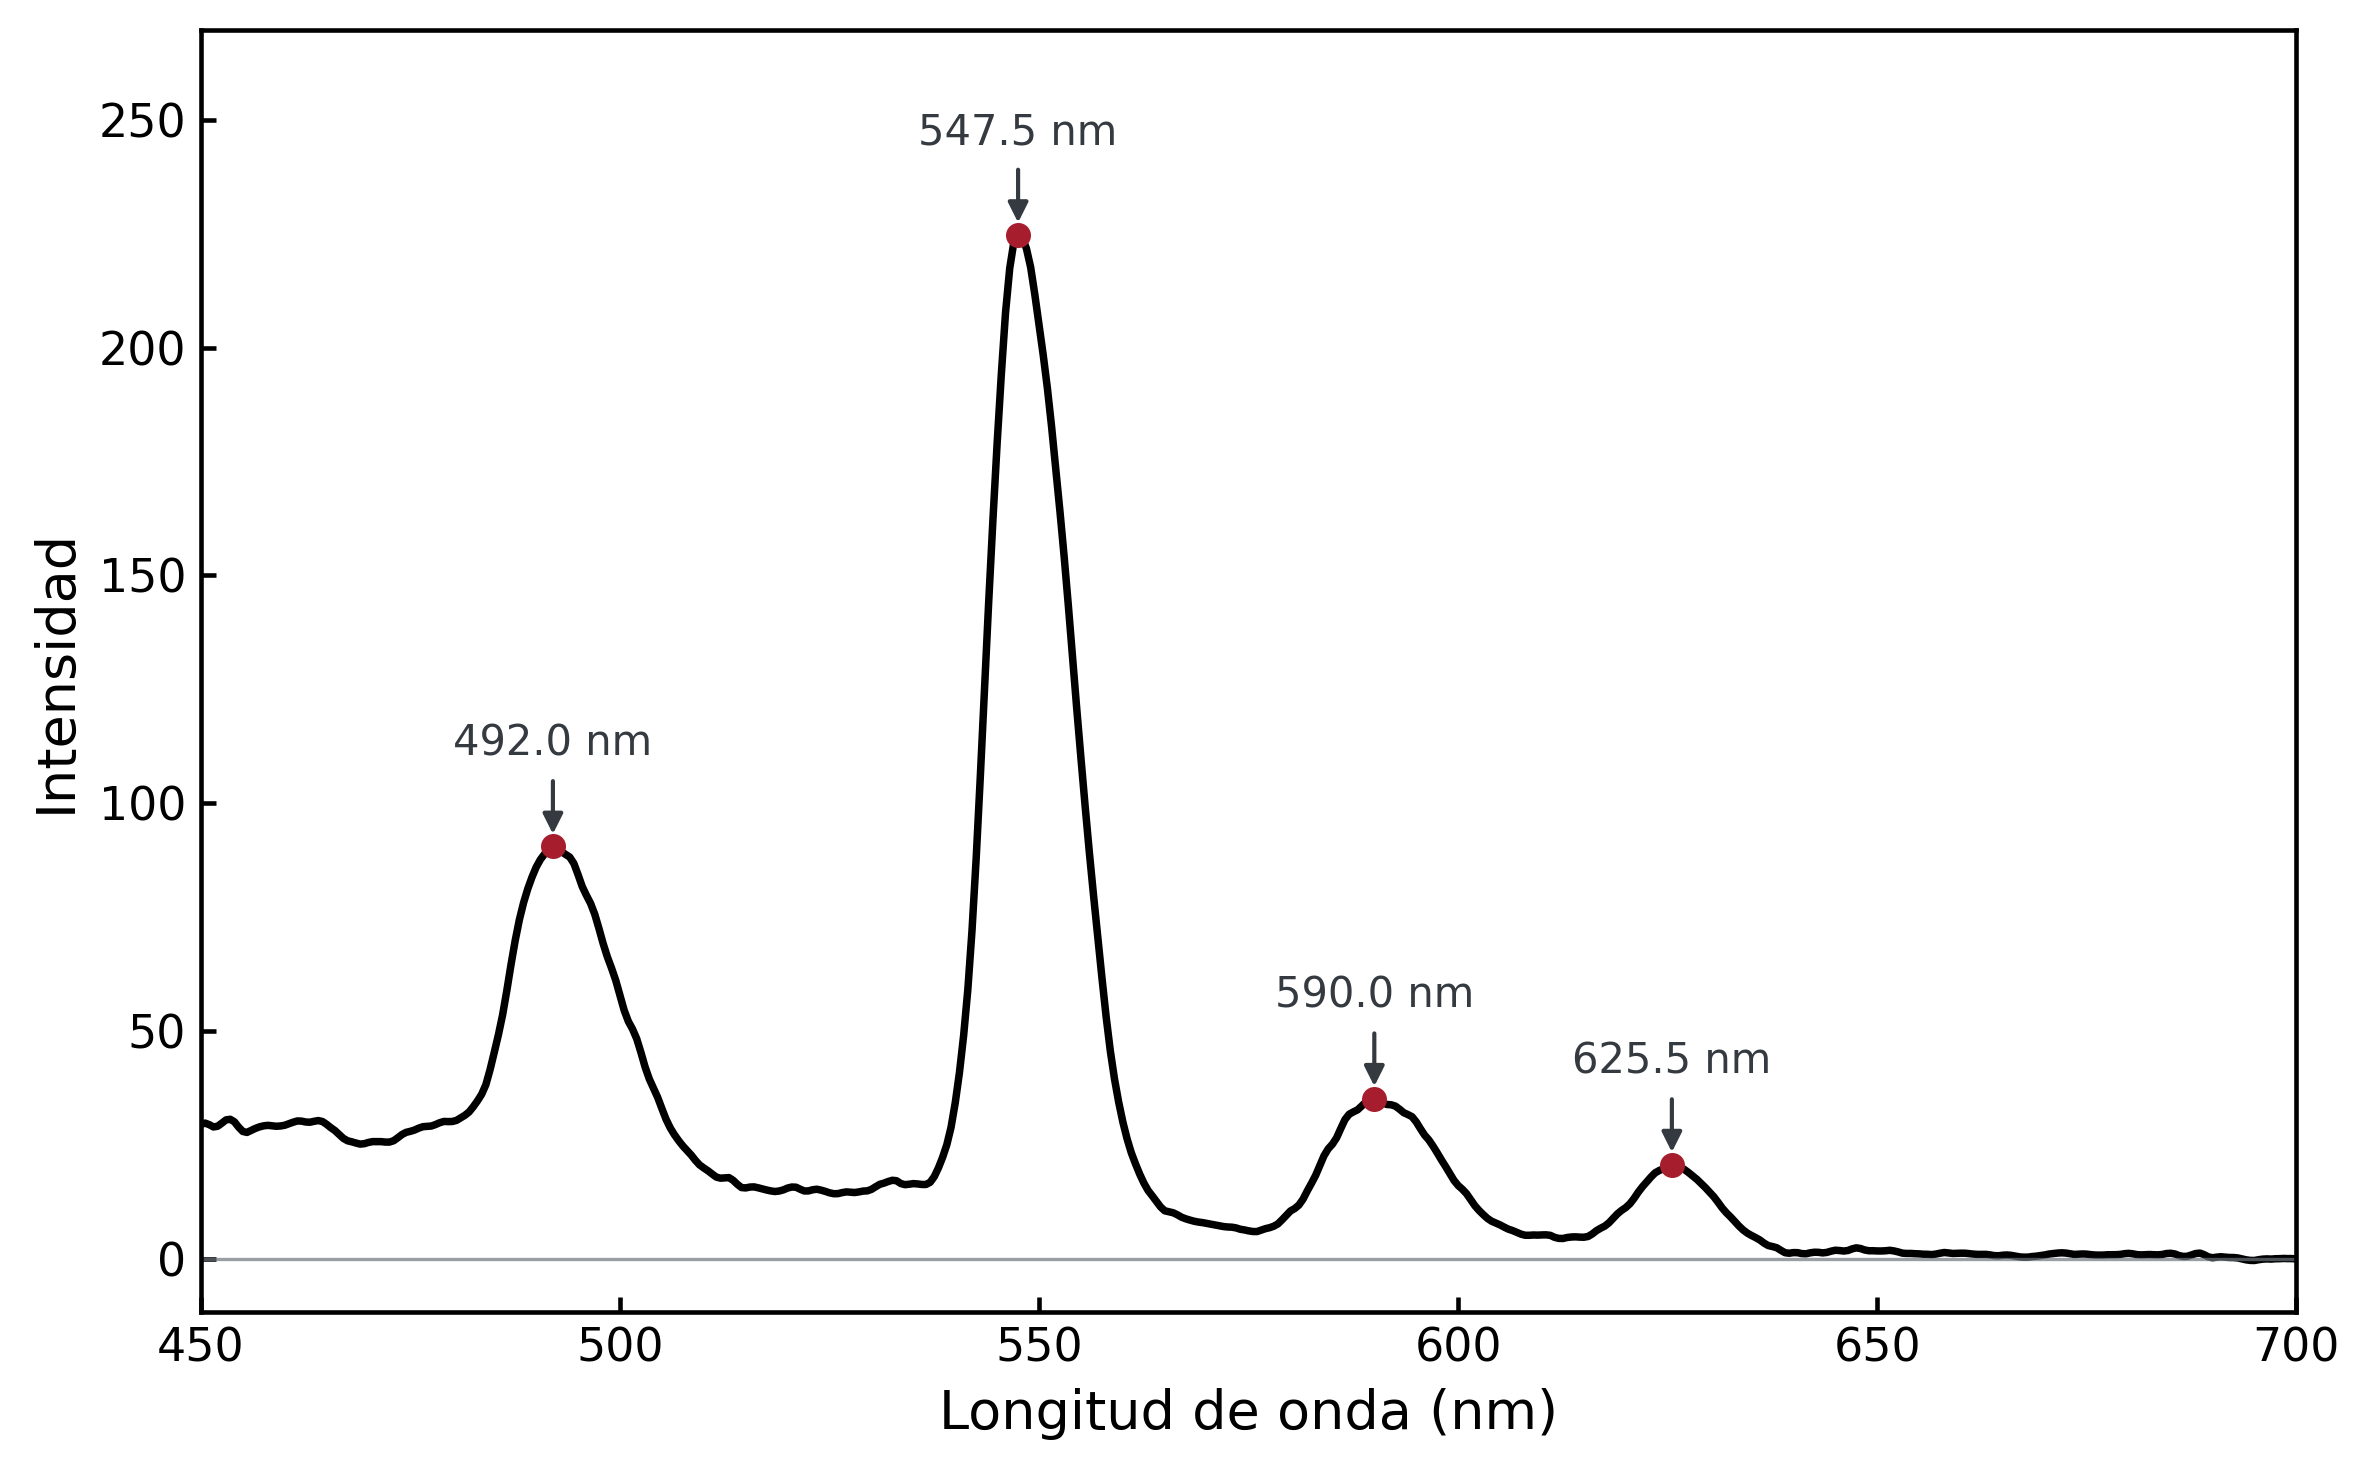
\includegraphics[scale=0.1]{figs/Tb_espec.png}
    \caption{Espectro de emisión de un cristal de Li$_2$B$_4$O$_7$ ($98\%$, composición molar) dopado con Tb$_4$O$_7$ ($2\%$). Se señalan las intensidades máximas.}
    \label{fig:Tb_espectro}
\end{figure}

Se utilizó la Ecuación \ref{eq:numero_onda} y se
calcularon las siguientes energías: $E_{Tb_1} = 20325.20
\pm 1489.20\ \mathrm{cm}^{-1}$, $E_{Tb_2} = 18264.84
\pm 767.63\ \mathrm{cm}^{-1}$, $E_{Tb_3} = 116949.15
\pm 948.75\ \mathrm{cm}^{-1}$ y $E_{Tb_4} = 15987.21
\pm 639.23\ \mathrm{cm}^{-1}$. Finalmente, para
la elaboración del diagrama de energía de este ion (Figura
\ref{fig:Tb_diagrama-ener}) se consideraron el rango de
las incertidumbres de la energía, y se eligió el que mejor
correspondía con la información disponible
actualmente. \cite{Tb-literatura}

\begin{figure}%[H]
    \centering
    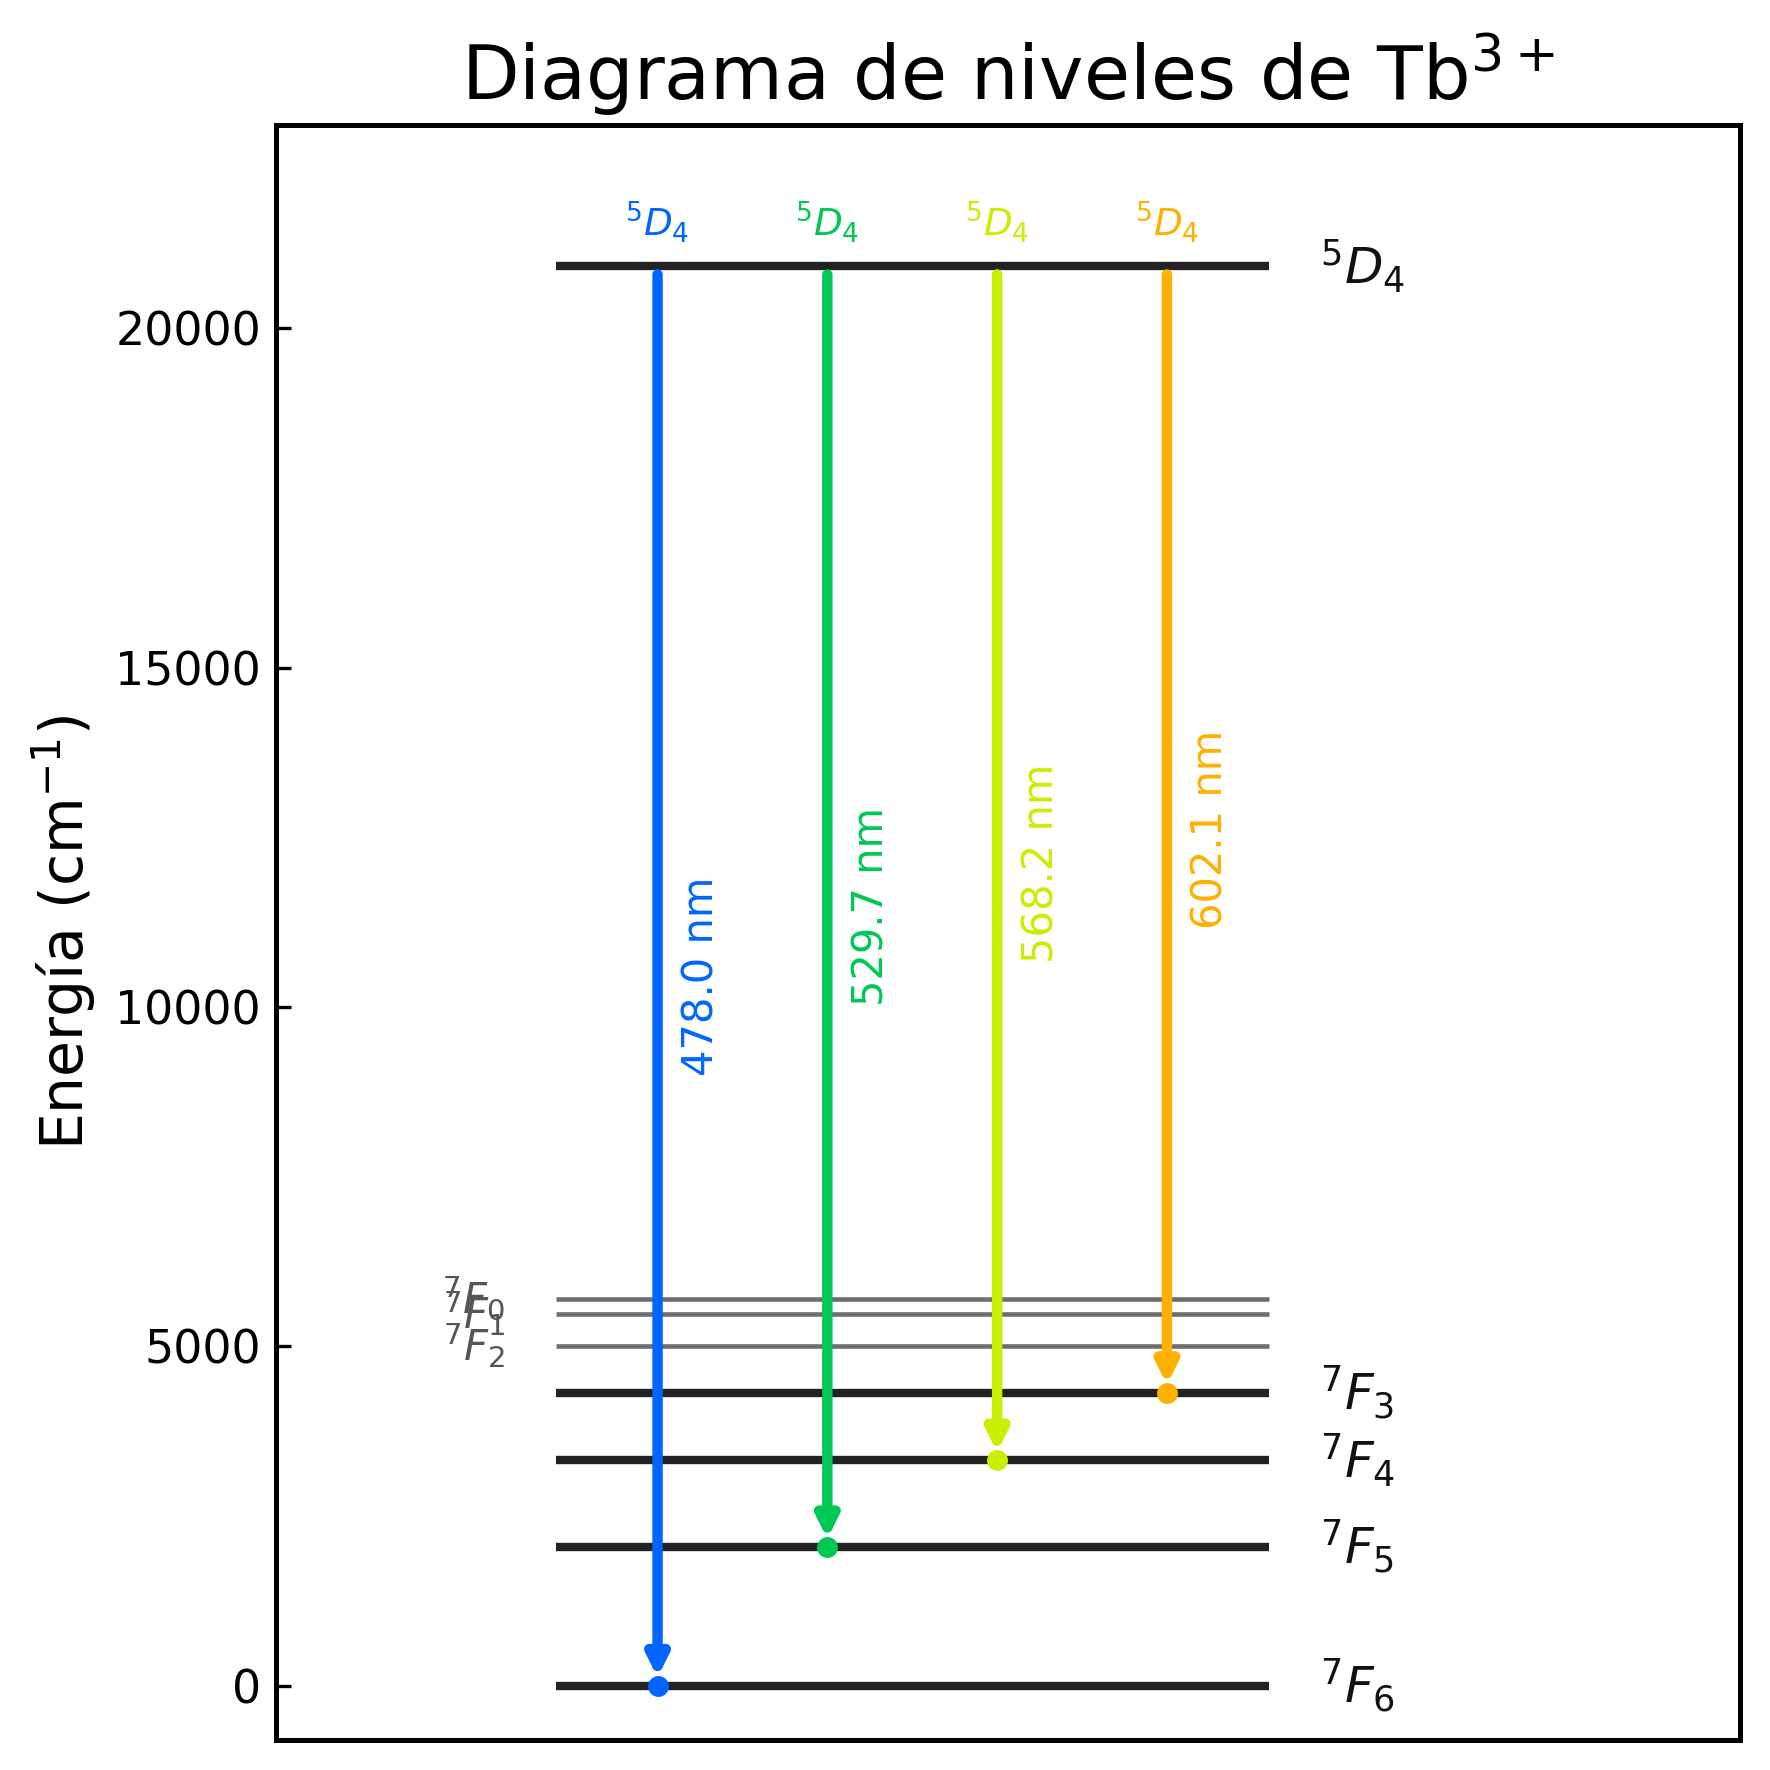
\includegraphics[scale=0.11]{figs/Tb-diag_ener.png}
    \caption{Diagrama de los niveles de energía de transición (fotoluminiscencia) del $Tb^{3+}$ calculado a partir de las intesidades máximas del espectro de emisión de un cristal de Li$_2$B$_4$O$_7$ ($98\%$, composición molar) dopado con Tb$_4$O$_7$ ($2\%$). Se señalan las longitudes de onda correspondientes.}
    \label{fig:Tb_diagrama-ener}
\end{figure}

%%%%% EUROPIO %%%%%%%%%%%%%%%%%%%%%%%%%%%%%%%%%%%%%%%%%%%%%

{\subsection{Europio en un cristal de metafosfato y ortofosfato de magnesio con cloruro de estaño}
\noindent En la Figura \ref{fig:Eu_espectro} se muestra su espectro de emisión. Se consideraron como bandas de mayor intensidad a las intensidades máximas de la gráfica más una incertidumbre, calculada como el ancho de la mitad de la intensidad máxima correspondiente. Por tanto, se obtuvieron los siguientes valores: $\lambda_{Eu_1} = 611.52 \pm 5.21$ nm, $\lambda_{Eu_2} = 592.02 \pm 13.28$ nm, $\lambda_{Eu_3} = 701.71 \pm 7.40$ nm y $\lambda_{Eu_4} = 653.22 \pm 24.62$ nm.

\begin{figure}%[H]
    \centering
    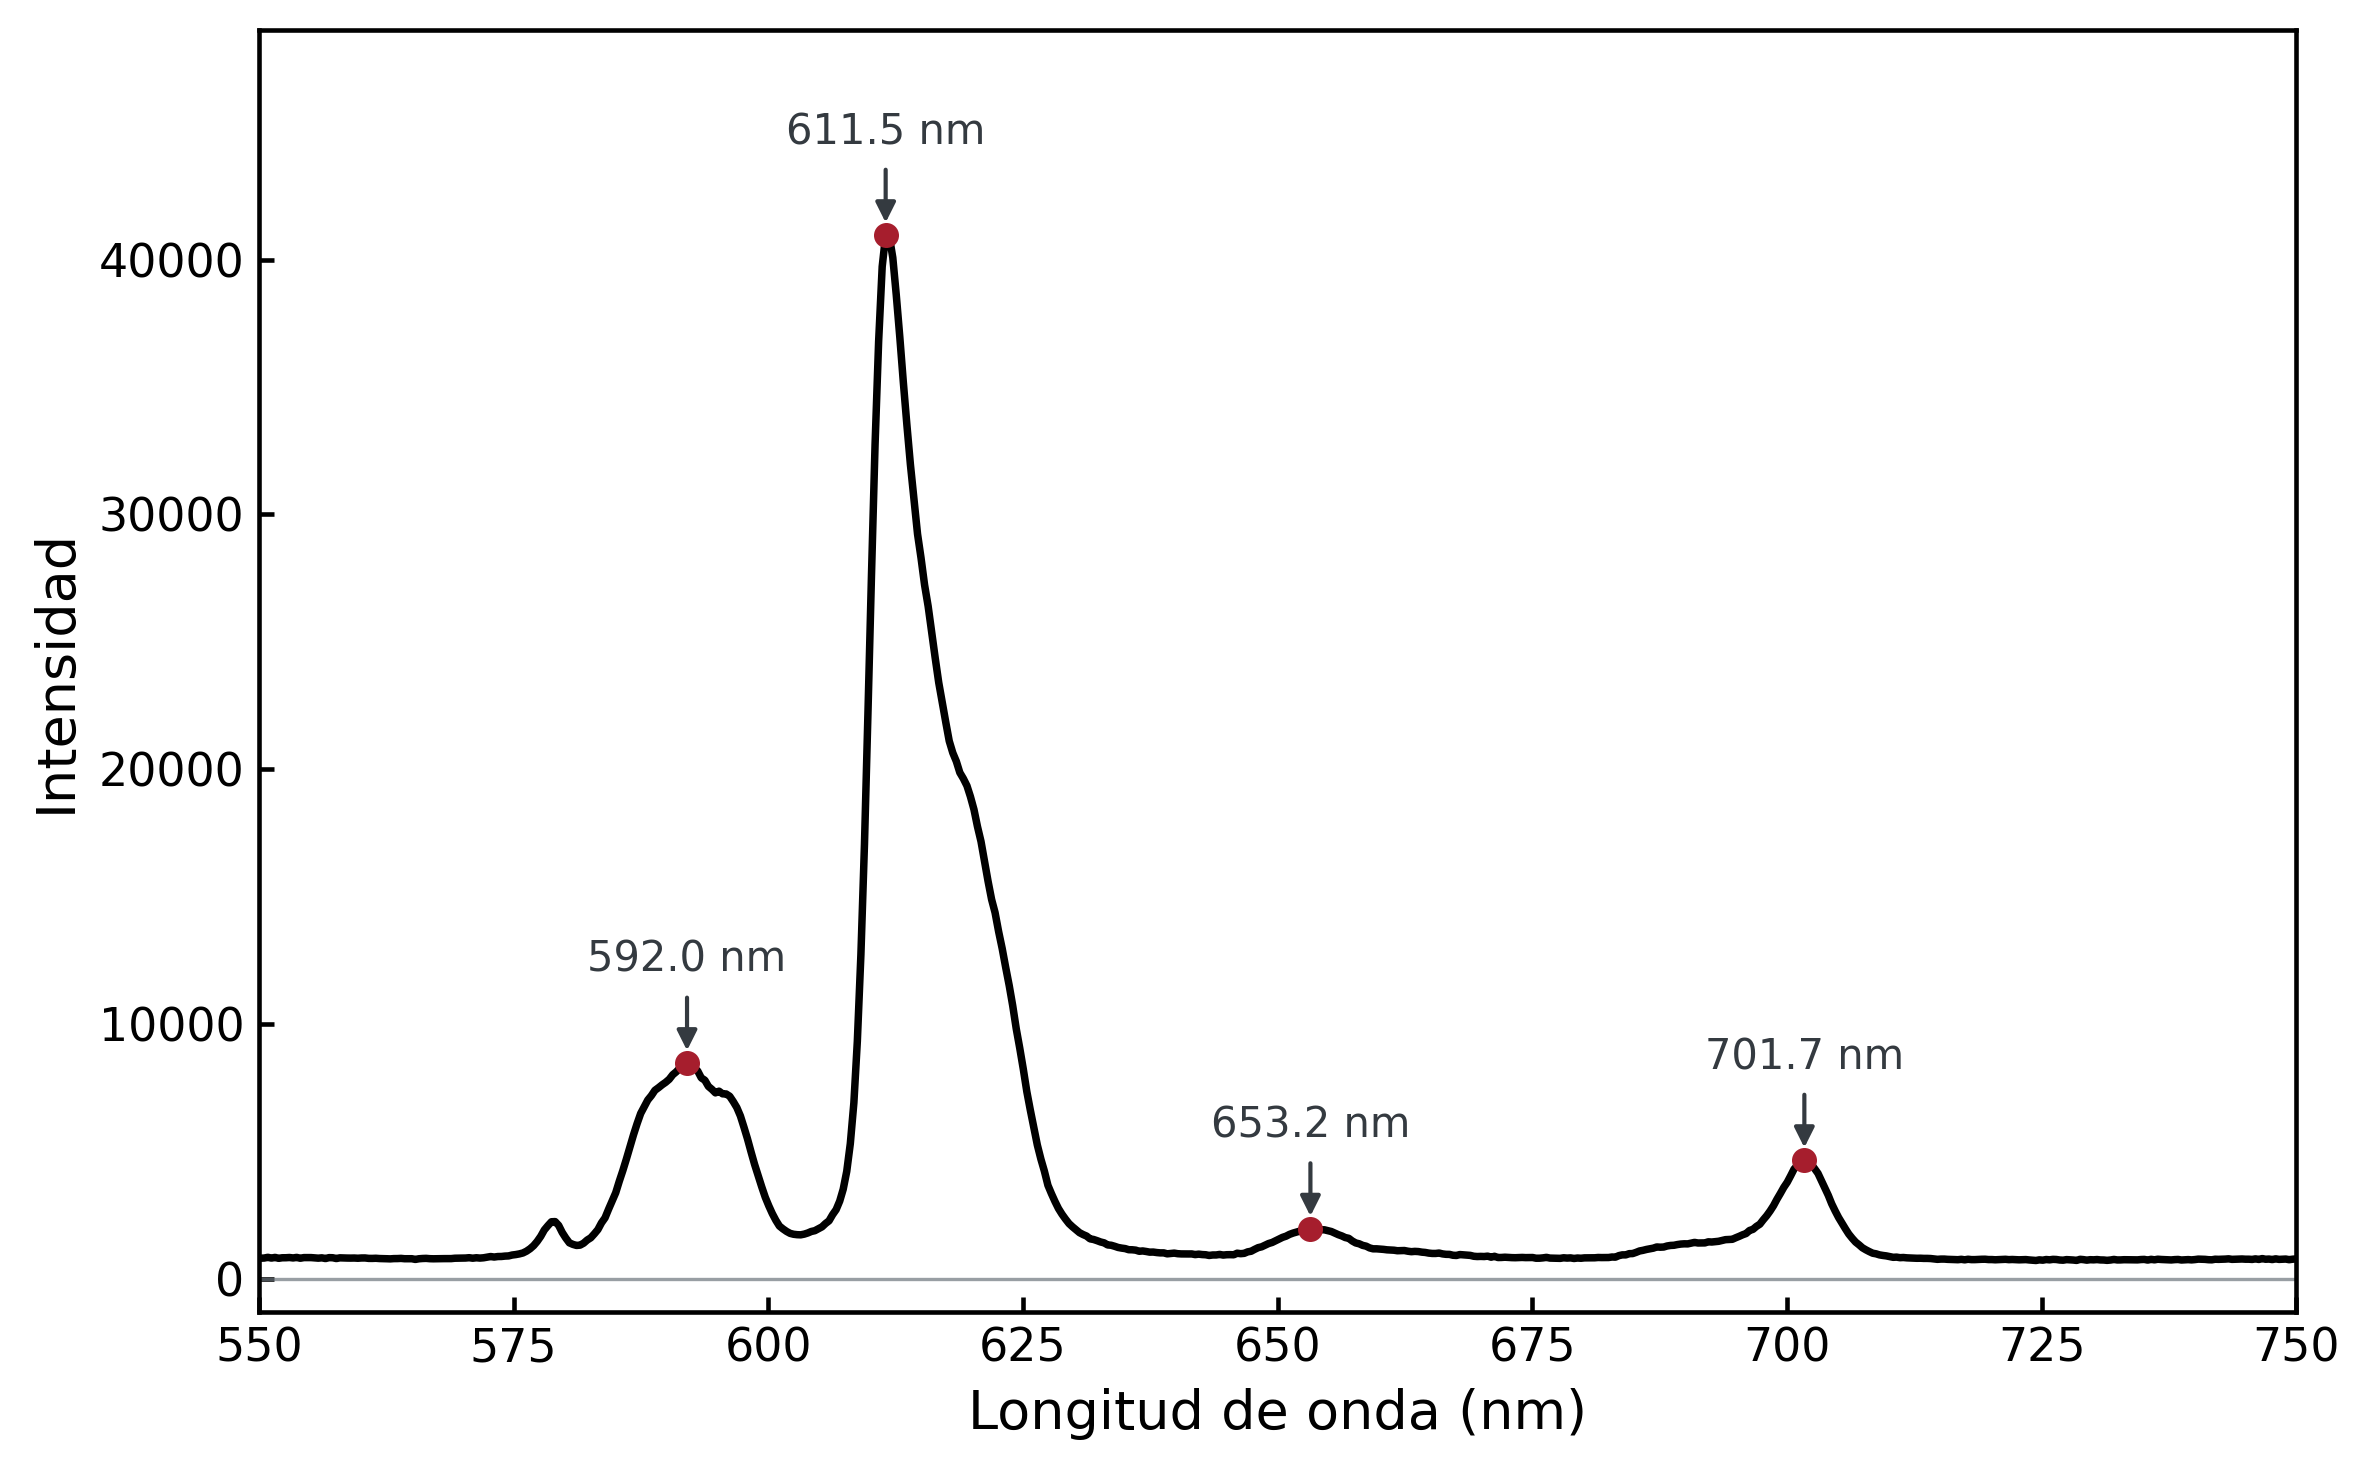
\includegraphics[scale=0.1]{figs/Eu-espec.png}
    \caption{Espectro de emisión de un cristal de Mg(PO$_3$)$_2$:Mg$_3$(PO$_4$)$_2$:SnCl$_3$ ($49\%$, $48\%$, $1\%$, composición molar) dopado con Eu$_2$O$_3$ ($3\%$). Se señalan las intensidades máximas.}
    \label{fig:Eu_espectro}
\end{figure}

Se utilizó la Ecuación \ref{eq:numero_onda} y se
calcularon las siguientes energías: $E_{Eu_1} = 16352.69
\pm 278.66\ \mathrm{cm}^{-1}$, $E_{Eu_2} = 16891.32
\pm 758.18\ \mathrm{cm}^{-1}$, $E_{Eu_3} = 14250.90
\pm 300.60\ \mathrm{cm}^{-1}$ y $E_{Eu_4} = 15308.78
\pm 1155.62\ \mathrm{cm}^{-1}$. Finalmente,
para la elaboración del diagrama de energía de este ión
(Figura \ref{fig:Eu_diagrama-ener}) se consideraron el
rango de las incertidumbres de la energía, y se eligió el
que mejor correspondía con la información disponible
actualmente. \cite{Eu_Pr-literatura}

\begin{figure}%[H]
    \centering
    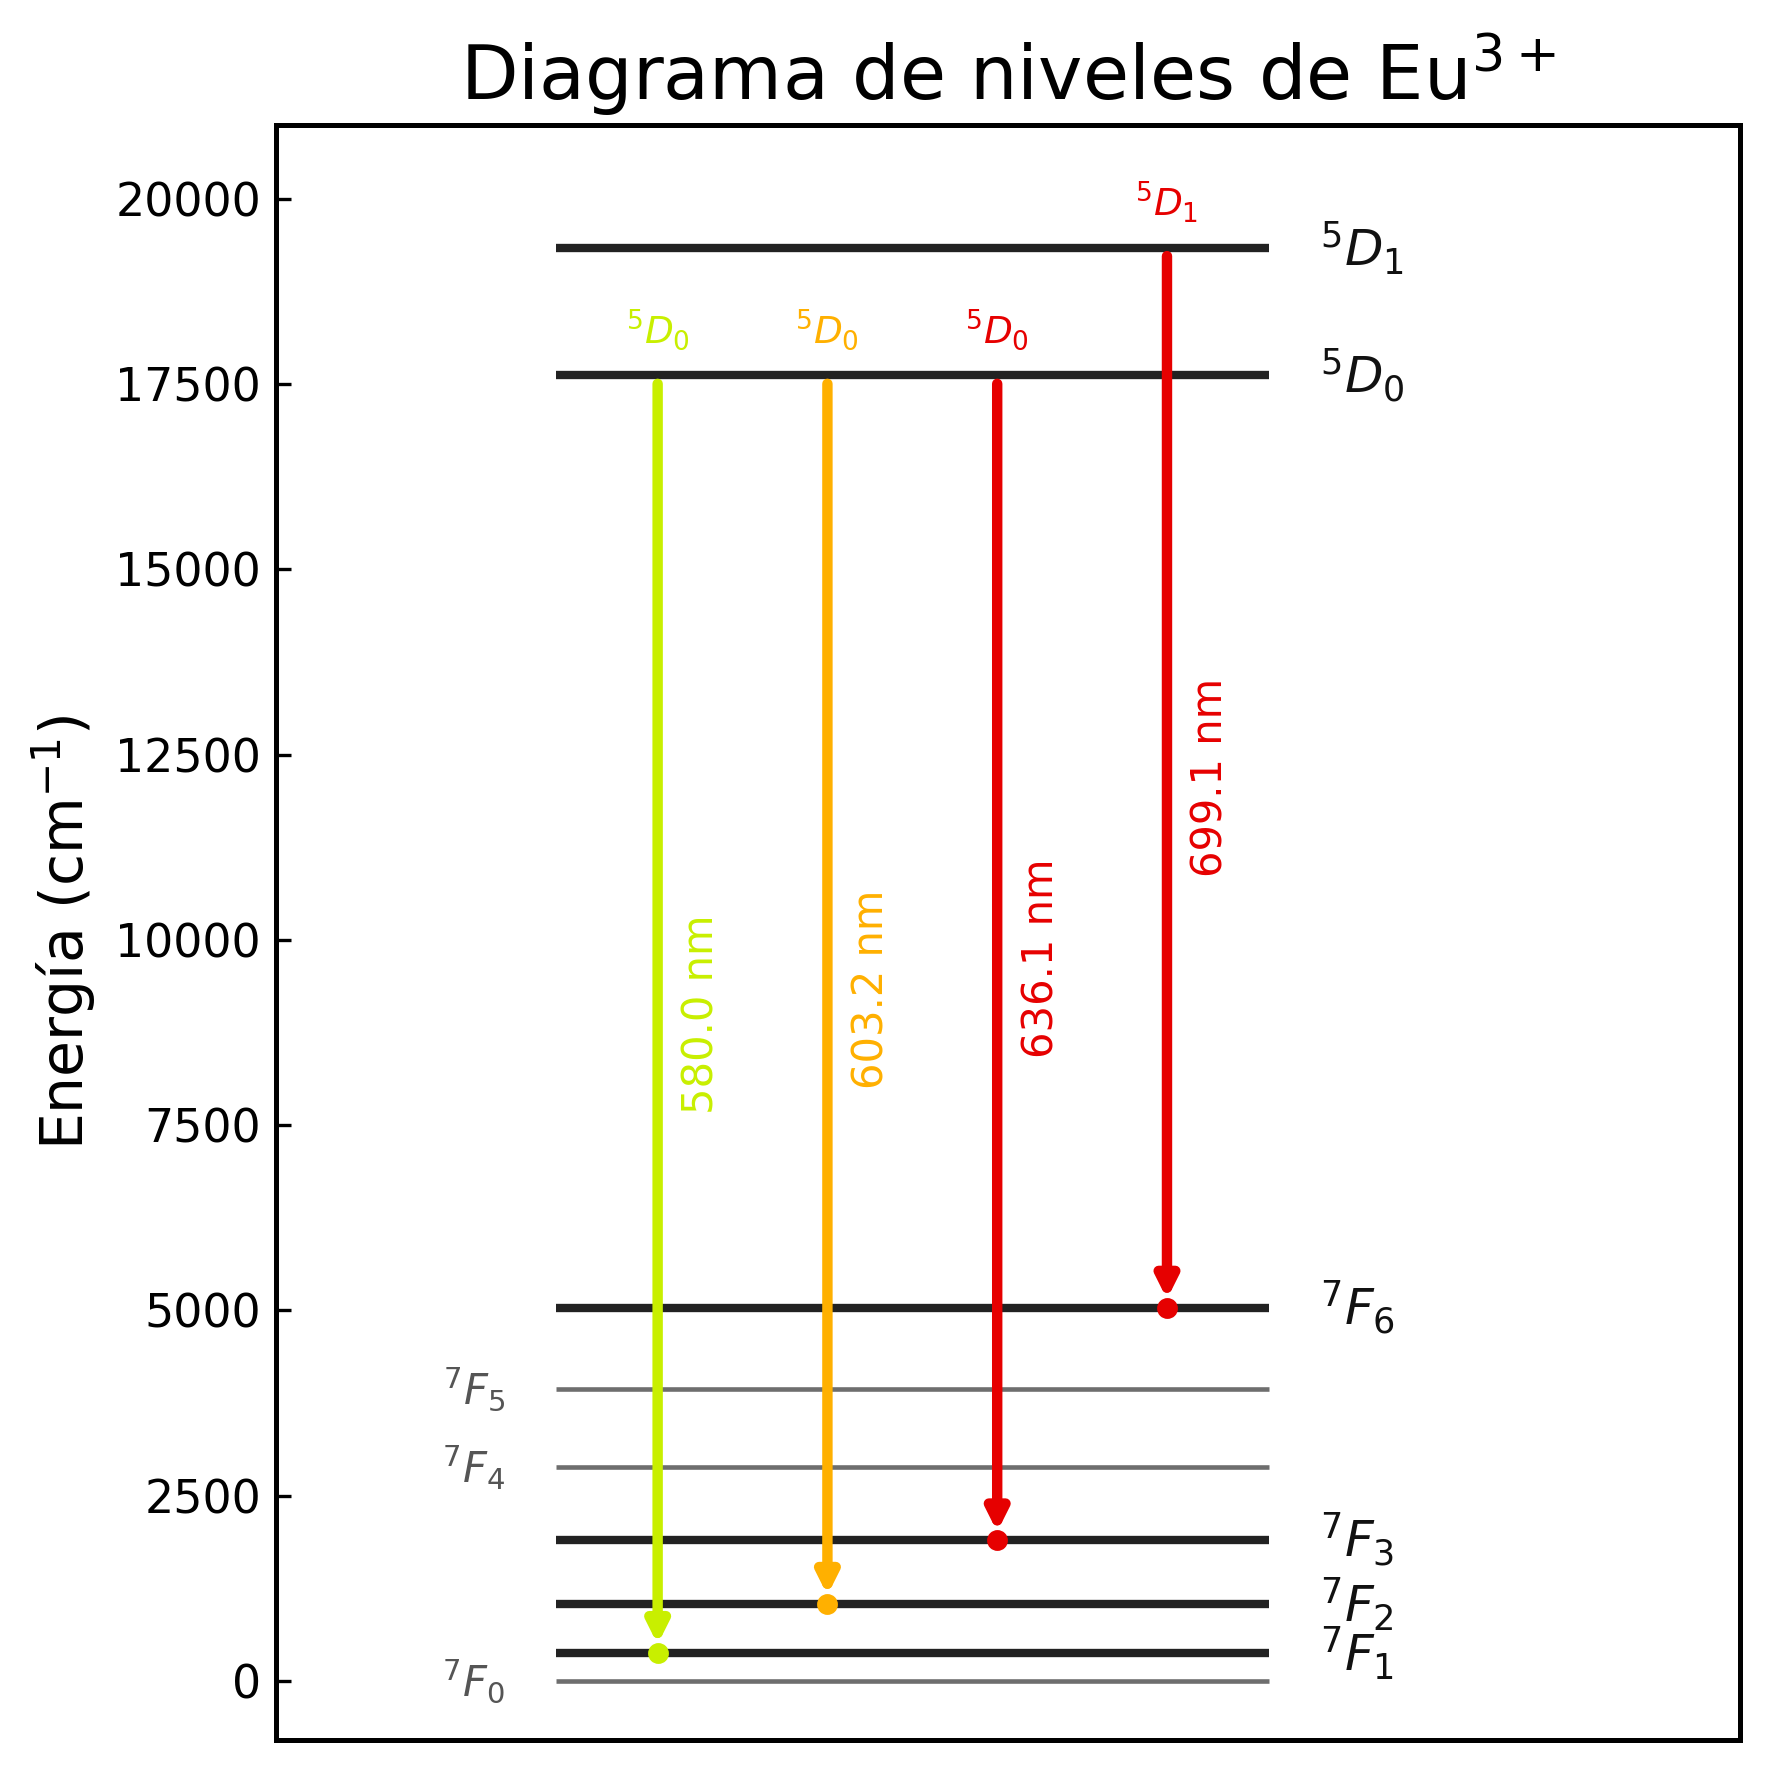
\includegraphics[scale=0.11]{figs/Eu-diag_ener.png}
    \caption{Diagrama de los niveles de energía de transición (fotoluminiscencia) del $Eu^{3+}$ calculado a partir de las intesidades máximas del espectro de emisión de un cristal de Mg(PO$_3$)$_2$:Mg$_3$(PO$_4$)$_2$:SnCl$_3$ ($49\%$, $48\%$, $1\%$, composición molar) dopado con Eu$_2$O$_3$ ($3\%$). Se señalan las longitudes de onda correspondientes.}
    \label{fig:Eu_diagrama-ener}
\end{figure}

%%%%% PRADEODIMIO %%%%%%%%%%%%%%%%%%%%%%%%%%%%%%%%%%%%%%%%%

{\subsection{Praseodimio en un cristal de metafosfato y ortofosfato de zinc}
\noindent En la Figura \ref{fig:Pr_espectro} se muestra su espectro de emisión. Se consideraron como bandas de mayor intensidad a las intensidades máximas de la gráfica más una incertidumbre, calculada como el ancho de la mitad de la intensidad máxima correspondiente. Por tanto, se obtuvieron los siguientes valores: $\lambda_{Pr_1} = 609.44 \pm 23.96$ nm, $\lambda_{Pr_2} = 640.88 \pm 8.59$ nm, $\lambda_{Pr_3} = 490.49 \pm 18.02$ nm, $\lambda_{Pr_4} = 525.64 \pm 30.25$ nm y $\lambda_{Pr_5} = 723.12 \pm 1.00$ nm.

\begin{figure}%[H]
    \centering
    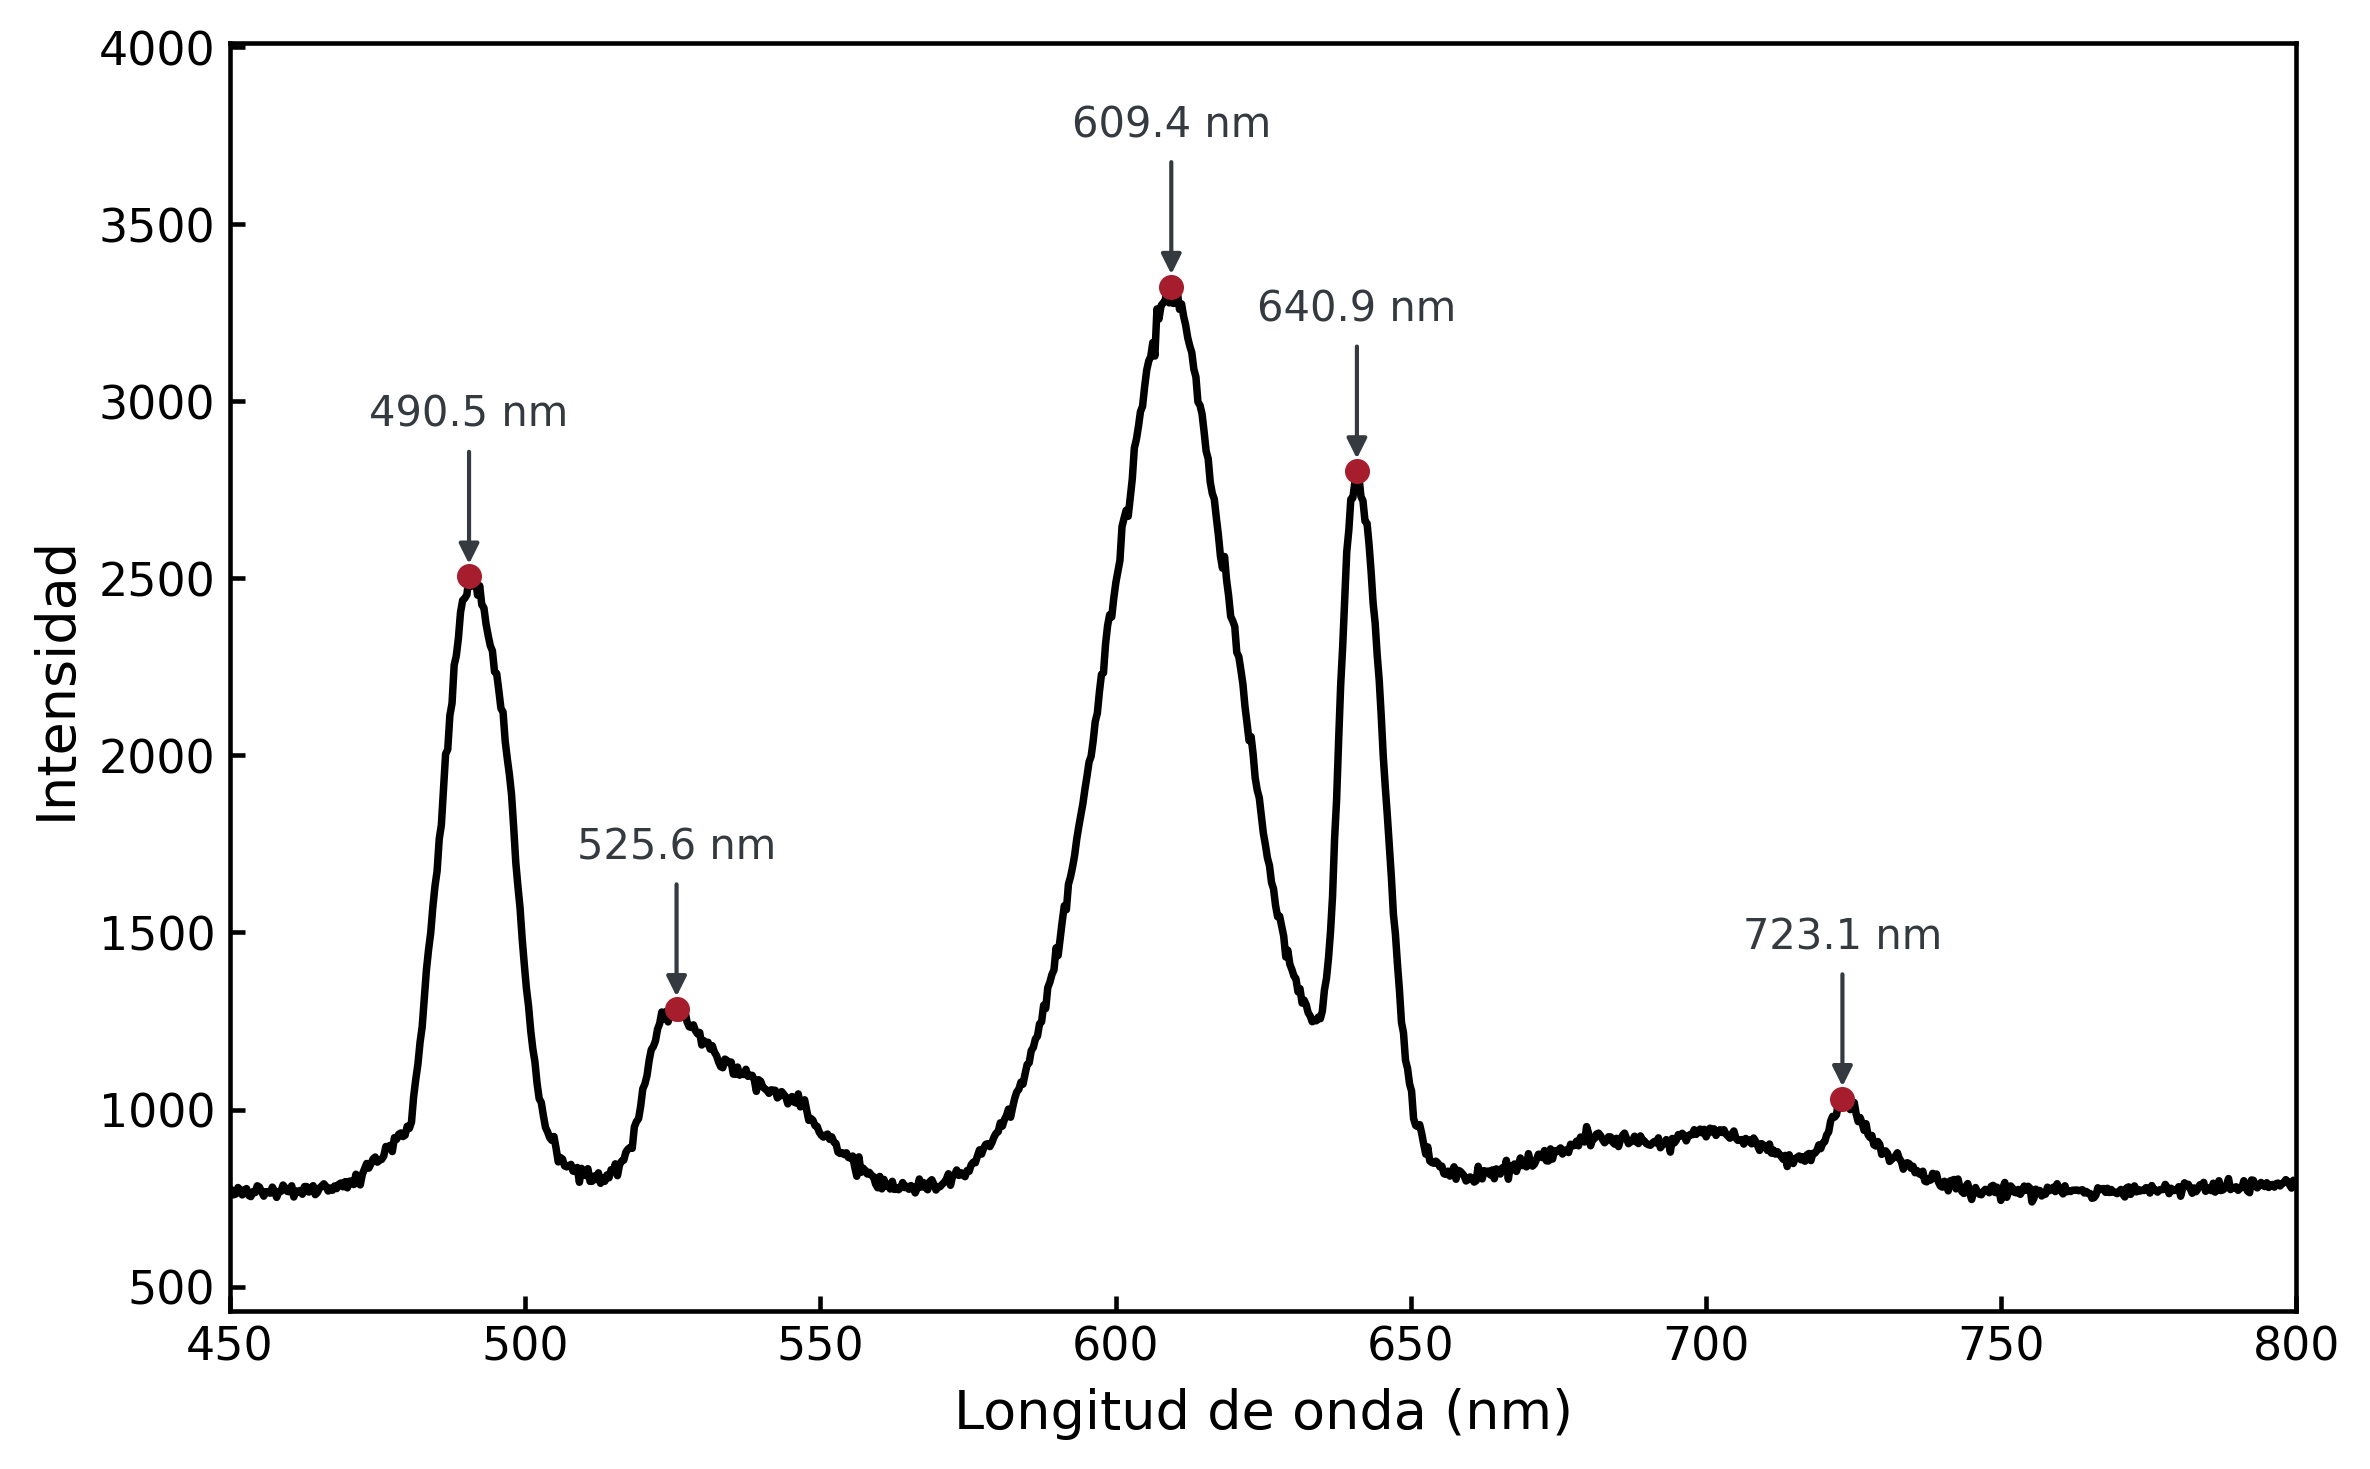
\includegraphics[scale=0.1]{figs/Pr-espec.png}
    \caption{Espectro de emisión de un cristal de Zn(PO$_3$)$_2$:Zn$_3$(PO$_4$)$_2$ ($49\%$, $49\%$, composición molar) dopado con Pr$_2$O$_3$ ($2\%$). Se señalan las intensidades máximas.}
    \label{fig:Pr_espectro}
\end{figure}

Se utilizó la Ecuación \ref{eq:numero_onda} y se
calcularon las siguientes energías: $E_{Pr_1} = 16408.51
\pm 1292.19\ \mathrm{cm}^{-1}$, $E_{Pr_2} = 15603.55
\pm 418.36\ \mathrm{cm}^{-1}$, $E_{Pr_3} = 20387.78
\pm 1500.07\ \mathrm{cm}^{-1}$, $E_{Pr_4} = 19024.43
\pm 2196.95\ \mathrm{cm}^{-1}$ y $E_{Pr_5} = 13828.96
\pm 48.25\ \mathrm{cm}^{-1}$. Finalmente,
para la elaboración del diagrama de energía de este ión
(Figura \ref{fig:Pr_diagrama-ener}) se consideraron el
rango de las incertidumbres de la energía, y se eligió el
que mejor correspondía con la información disponible
actualmente. \cite{Eu_Pr-literatura}

\begin{figure}%[H]
    \centering
    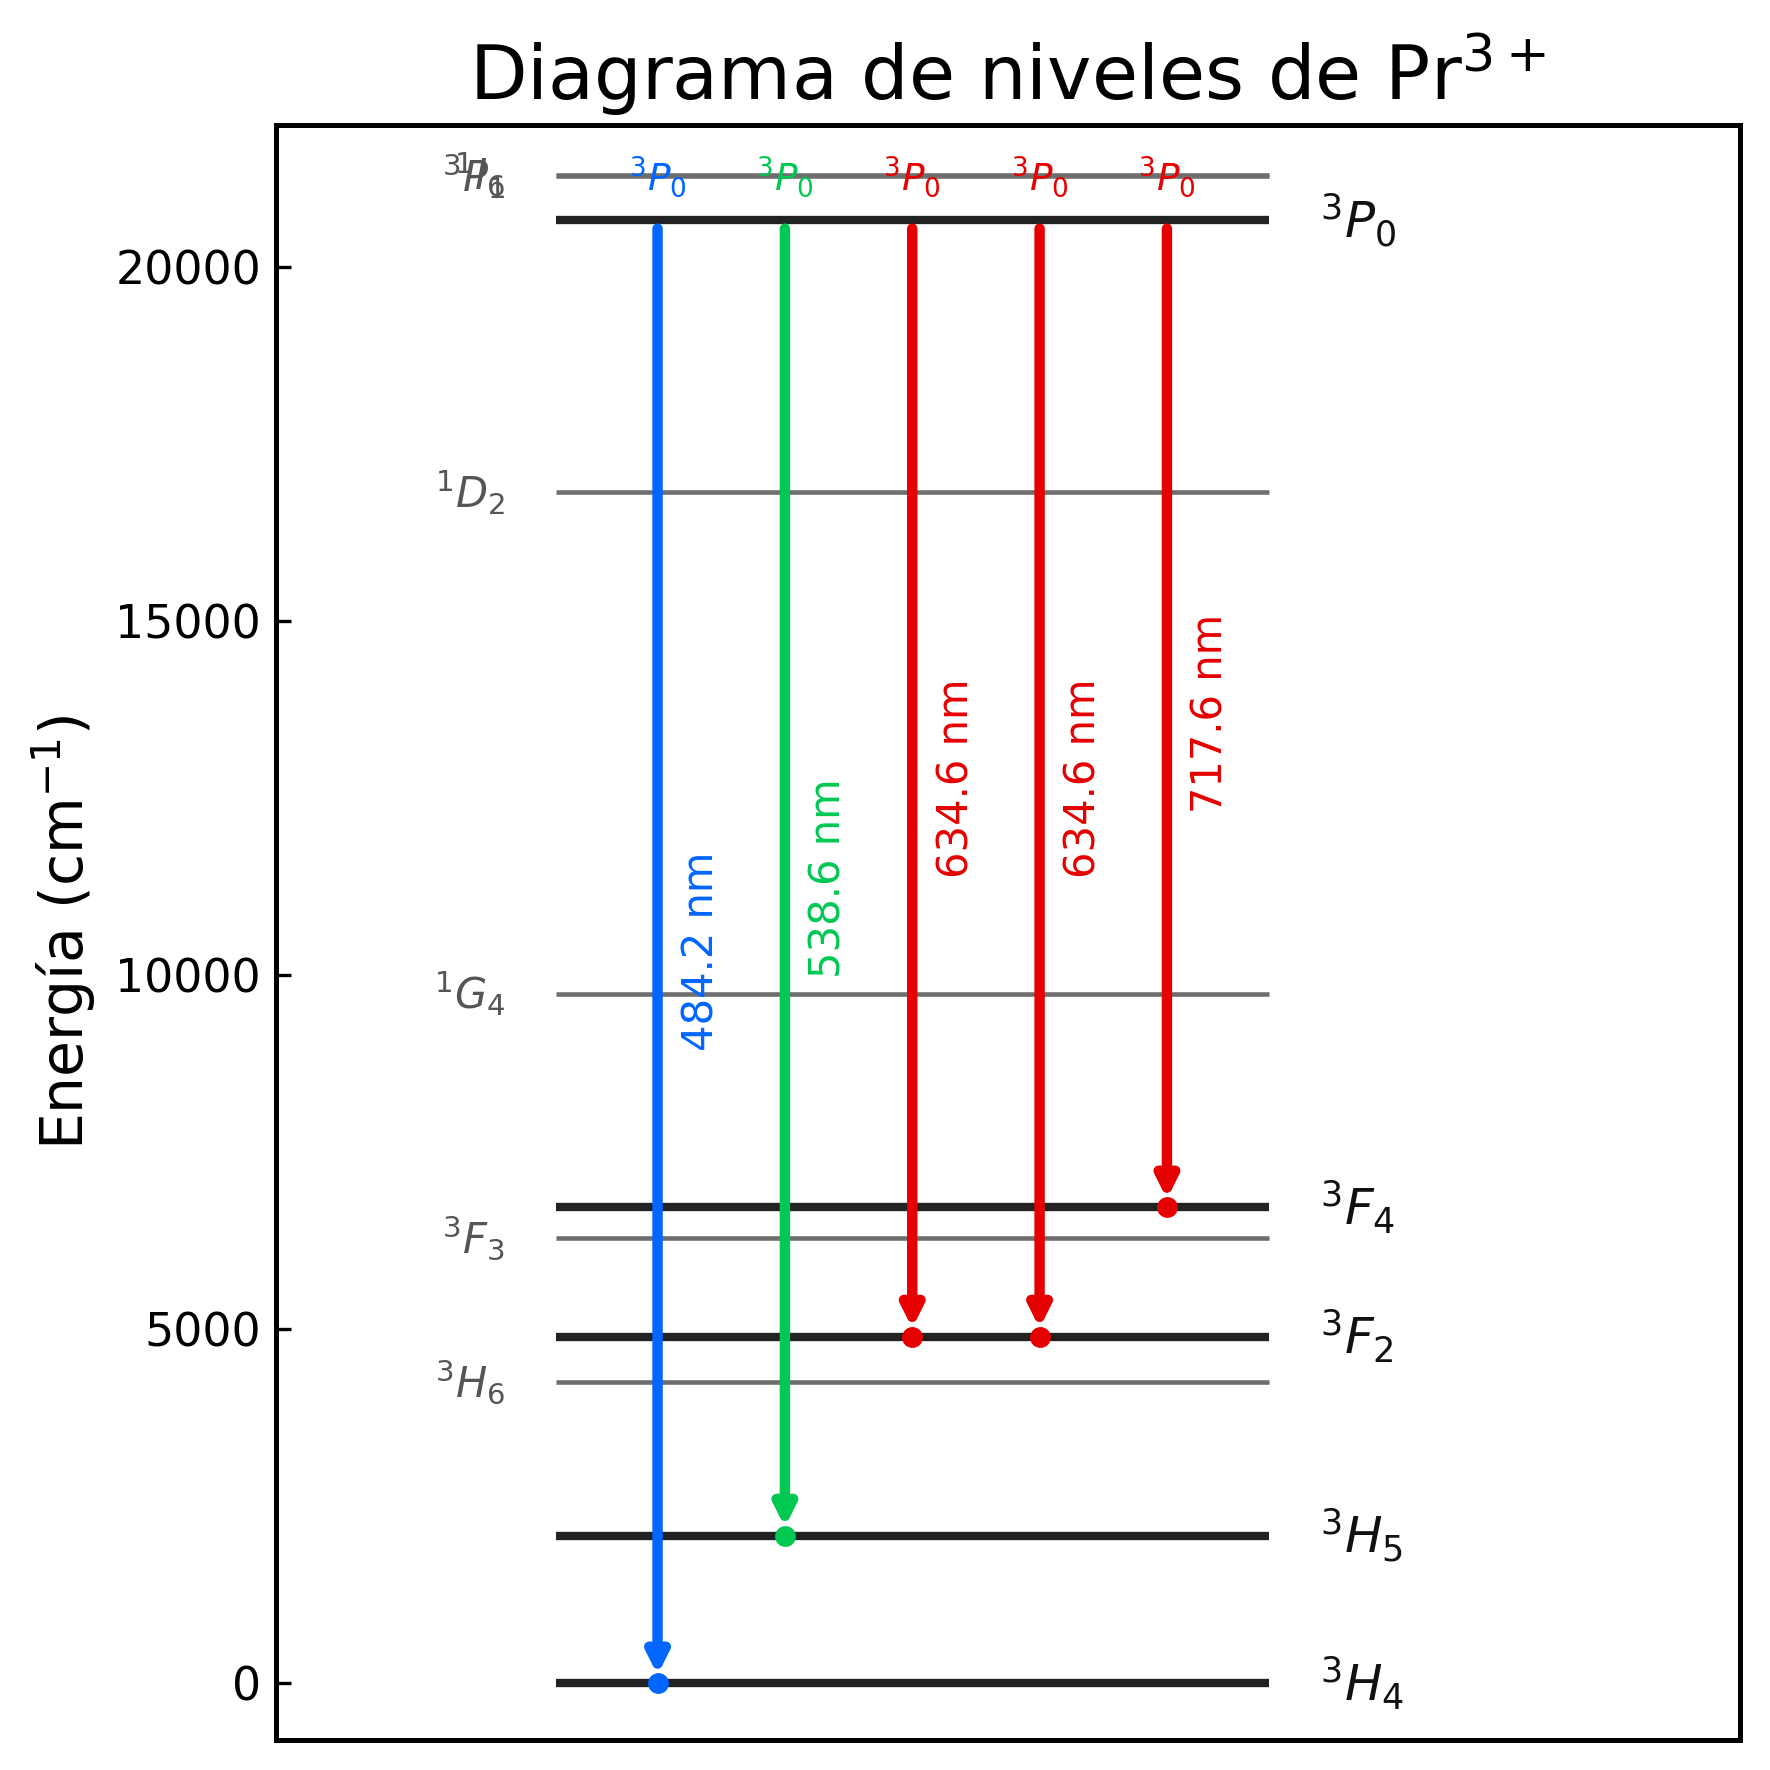
\includegraphics[scale=0.11]{figs/Pr-diag_ener.png}
    \caption{Diagrama de los niveles de energía de transición (fotoluminiscencia) del $Pr^{3+}$ calculado a partir de las intesidades máximas del espectro de emisión de un cristal de Zn(PO$_3$)$_2$:Zn$_3$(PO$_4$)$_2$ ($49\%$, $49\%$, composición molar) dopado con Pr$_2$O$_3$ ($2\%$). Se señalan las longitudes de onda correspondientes.}
    \label{fig:Pr_diagrama-ener}
\end{figure}